\documentclass[10pt,a4paper]{article}

\usepackage[utf8x]{inputenc}
\usepackage{ucs}
\usepackage[francais]{babel}
\usepackage[T1]{fontenc}

\usepackage{amsmath}
\usepackage{amsfonts}
\usepackage{amssymb}

\author{LAFON Sylvain, MAINGRET François et LEVASSEUR Thomas}
\title{Rapport - Bob-Project}

\begin{document}

	\maketitle
	\tableofcontents
	\newpage
	\part{Objectif}
		L'objectif de ce projet était de réaliser un site web pour un magasin de bricolage, Brico-Bob.  Ce site devra gérer plusieurs aspects : une partie privée et une partie publique. La partie publique sera accessible a n'importe qui, et comprendra, entre autres, la possibilités de visionner des produits, d'en rechercher, de commenter un produit. La partie privée sera réservée aux administrateurs du site et comprendra un panneau permettant de gérer tout le contenu du site, des produits, images, catégories...  
		\section{Objectifs du site}
		L'objectif de notre site est de proposer à la vente comme à la location des articles de bricolage pour le grand public.  Le site devra donc être assez ergonomique et  attrayant visuellement afin de ne pas repousser les visiteurs.\\
		
Voila les points importants sur lesquels sur lesquels nous avons fait attention :
			\begin{itemize}
\item Un temps de chargement des pages optimisé. En effet On estime le seuil d'acceptation de chargement d'un site à deux secondes (selon plus de 47\%  des internautes sondés).  Au delà, vous commencez à perdre des visiteurs. ( source : Marketing Management par  P. Kotler ).\\

\item Proposer une description des produits assez détaillée : si le client ne trouve 	pas 	assez d'informations sur un produit sur notre site, il ira chercher ces 	informations chez un concurrent, et a moins que notre prix soit 	significativement plus bas, il y a de grandes chances qu'il achète chez ce 	concurrent.\\

	
\item Il faudra utiliser le plus de termes simples a comprendre par l'utilisateur plutôt 	que des termes techniques barbares.  Notre site permet donc d'écrire de 	longues description, mais cette responsabilité incombe plutôt à la société Brico-	Bob.\\

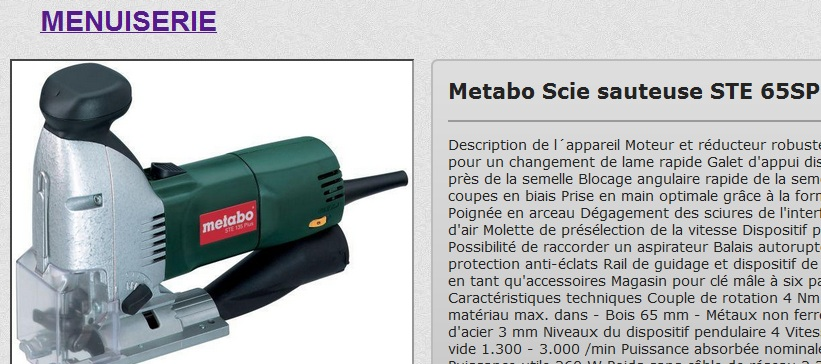
\includegraphics[scale=0.5]{demofichepro.jpg}

\item Donner des informations sur la société et sur le service client, ainsi que les 	administrateurs du site. Le client veut savoir a qui il a affaire et sera plus enclin 	à acheter si il sait qu'il peut contacter quelqu'un ensuite. Le client sera mis en 	confiance, ce qui est vraiment important lorsque son argent est en jeu.\\
	Ces informations seront donc accessibles depuis n'importe quelle page du site 	grâce au menu :\\

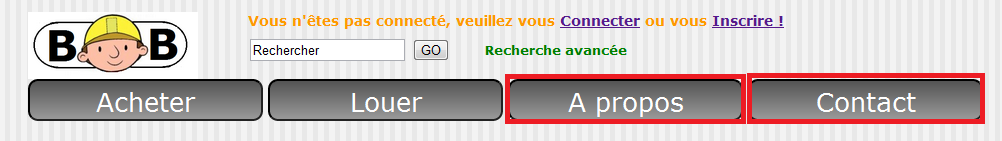
\includegraphics[scale=0.5]{menu.jpg}

\item Ne pas trop s'introduire dans la vie privée du client : nous n'avons demandé 	au client que des informations non personnelles lors de son inscription :  son 	pseudo et un mot de passe. Il n'as pas besoin de donner son nom ni son 	adresse tant qu'il ne valide pas une commande. Cela lui permettra de ne pas se  	sentir "tracké" et de visiter librement le site.\\

\item Un moteur de recherche bien réalisé. Si le client sait exactement ce qu'il veut 	lorsqu'il va sur le site, il ira chercher le nom du produit qu'il a en tête dans la 	barre de recherche. Si le moteur de recherche n'est pas bien conçu, il risque de 	penser que nous n'avons pas le produit qu'il cherche et il ira donc voir ailleurs. 	Si il n'a qu'une idée très vague, il y a alors des chances qu'il se tourne vers le 	moteur de recherche avancée. Cela nous permettra de cerner ses critères de 	prix par exemple.\\

\item Mettre en évidence le produit en mettant une image assez grande : trop de site proposent encore des images ridiculement petites, ce qui peut décourager le client d'acheter, car il ne peut pas bien voir le produit et peut même penser qu'il y a des risques de "tromperie" sur la marchandise.\\

\item Une navigation aisée, c'est à dire des catégories bien organisées. Bien que notre site permette d'afficher à la fois des produits et des catégories sur une même page, cela sera à éviter dans le cas général. Enfin, il faudra veiller à ne pas créer de catégories vides, qui prendrait de la place pour rien et serait une source de  frustration pour le client ( quoi de plus désagréable que de trouver une catégorie qui correspond parfaitement à ce que l'on recherche et se rendre compte qu'elle est vide )\\

\item Mettre l'accent sur les produits : le but d'un site de e commerce est de vendre, et nous avons donc fait attention de mettre l'accent sur les produits. Le design est assez sobre, et les autres éléments du site 	n'empiètent as sur les produits. Il y a également sur la page d'accueil des "coups de cœur" permettant de stimuler un achat imprévu chez le client.


\end{itemize}
	
	\newpage
	\part{Organisation}
		\section{Introduction}
			\subsection{Au sein de l'equipe}
				\begin{itemize}
					\item François Maingret (rfk78) s'est occuppé du design du site.
					\item Sylvain Lafon (sylafrs) s'est occuppé du code principal du site.
					\item Thomas Levasseur (sion77) s'est occuppé du JavaScript du site.
				\end{itemize}
			\subsection{Support du code}
				Pour le projet nous avons utilisé plusieurs supports.\\
				Commençons par Github : il s'agit d'un système de partage de fichiers gratuit (si on les laisse opensource) très pratique.\\
				Nous avons aussi utilisé l'éditeur de texte Notepad++ ainsi que l'émulateur Wamp (et Lamp parfois). Cet emulateur, comme l'indique son nom, permet d'emuler sur une machine un serveur Apache/MySql/Php pour pouvoir tester le site en local.\\
				Enfin, un certain nombre d'images, le logo, ou des éléments graphiques de l'interface ont été réalisées grâce à the GIMP. 
		\subsection{Langages}			
			Nous avons utilisé, comme pour la plupart des sites, les langages :
\begin{description}
	\item[HTML :] Utilisé pour la structure des pages web, elle permet de définir les éléments que contiens la page. On s'en est notamment servi pour organiser la page grâce aux balises <div> et <span>.
	
	\item[CSS :] Nous avons géré tout le design de notre site grâce a divers fichiers css, nous n'avons pas inséré de CSS directement dans le HTML.
Le design a été découpe en divers fichiers, chacun étant utile pour le design d'une partie du site. L' "assemblage" des fichiers .css nécessaires
se fait en partie grâce à SMARTY.
	
	\item[PHP :] Utilisé pour rendre le site interactif en iteragissant avec la base de données (avec le langage SQL) et en traitant les données.
	Php va ensuite appeler Smarty et lui passer des données pour afficher une page.\\
	Nous utilisons Php, notemment pour :
	\begin{itemize}
		\item Créer des comptes utilisateurs
		\item Gérer les sessions
		\item Utiliser un panneau administrateur afin de gérer le contenu du site
	\end{itemize}
	
	\item[SQL :] Toutes les catégories, membres, produits, avis sont stockées dans la base de donnée. Nous avons utilisé cette base de donnée pour stocker certaines images telles que les illustrations des produits mis à disposition. Ces installations ont nécessité un certains nombre de contrôle de sécurité mais 	ce sont elles qui permettent d'avoir un site fonctionnel.\\
	Le SQL permet de manipuler la base de données.\\
	On stockera les informations de la base dans les classes Php
	
	\item[JavaScript :] Le JavaScript sur notre site nous sert principalement à contrôler les entrées de l'utilisateur, par exemple sur la page d'inscription afin de contrôler que les informations entrées sont valides.
Nous l'utilisons donc dans certains formulaires du site afin de ne pas provoquer de trop grosse frustration chez l'utilisateur au cas ou il clique sur "valider"
en ayant entré des informations non valides.
Voila un autre exemple d'utilisation du JavaScript, qui permet de rentre le système de notation plus attractif : l'utilisateur note un produit en cliquant sur le
nombre d'étoiles qu'il souhaite lui attribuer.

\end{description}

		\subsection{Bibliothèques}
		
\begin{description}
	\item[AJAX :] Exploité par le JavaScript, il permet de recuperer une autre page et de traiter ces alors que la page ayant appelé AJAX est encore active.
Il permet, par exemple, alors que la page d'inscription est affichée, de demander au serveur si tel ou tel pseudo est utilisé ou non.

	\item[Smarty :] C'est un moteur de templates, il permet de séparer traitement des données et mise en page : L'index va commencer par analyser la requête, et suivant son analyse va appeler tel ou tel template en lui 'passant' des variables qu'il pourra alors utiliser pour l'affichage.
\end{description}
	\subsection{Base de donnée}
	La base de donnée nous a servi à stocker une très grande partie des données du site. Nous avons stocké :
	\begin{itemize}
	\item Les informations sur les membres et les administrateurs
	\item Les produits
	\item Les catégories et les sous catégories de produits
	\item Les avis sur les produits
	\item Les images d'illustration des catégories et des produits.
	\end{itemize}
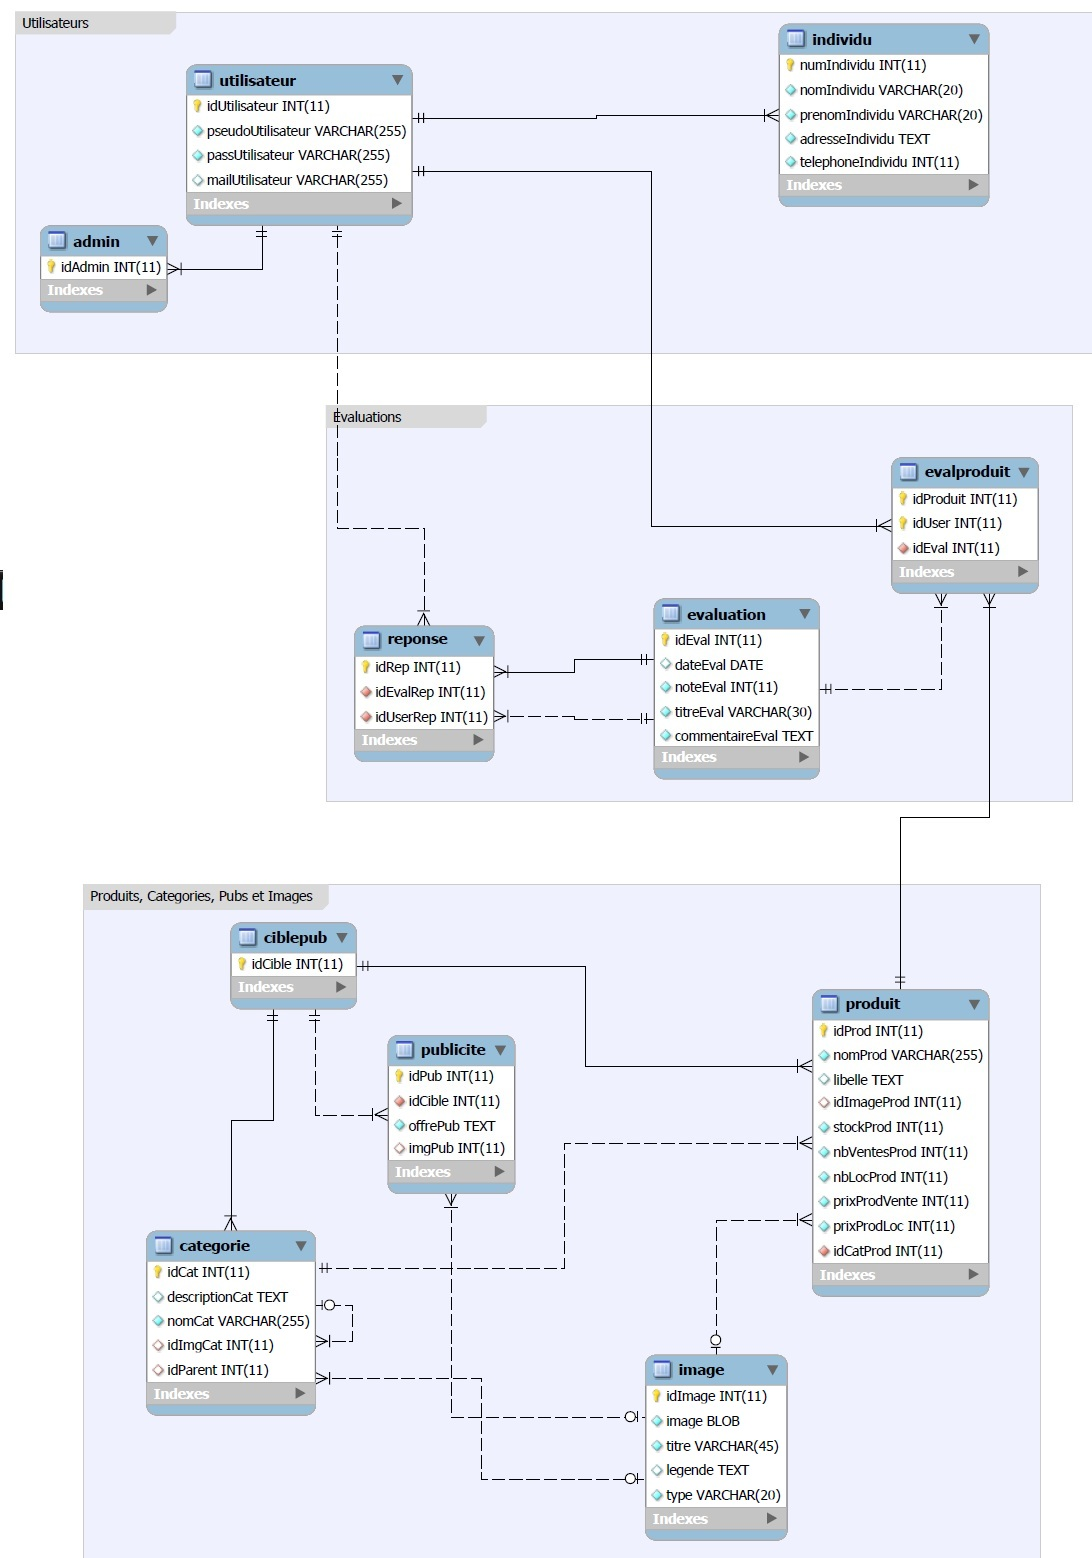
\includegraphics[scale=0.5]{dbob.jpg}	

		\section{Structure du code}
			\subsection{header.php}
				Ce fichier va inserer la bibliothèque Smarty et les déclarations de classes, puis il va déclarer des constantes et crée quelques fonctions  
			\subsection{index.php}
				Ce fichier va tout d'abord appeller header.php puis va creer l'objet Bob et smarty.\\
				Il va ensuite analyser la requete pour savoir quel template il va appeller pour fabriquer la page et va effectuer les actions qu'on lui demande de faire.\\
				Il va ensuite passer à smarty plusieurs variables puis generer la page.
			\subsection{les fichiers de /classes}
				Ces fichiers contiennent les classes qui contiennent les infos de la base de données et qui la manipule.
			\subsection{les fichiers de /templates}
				Ils permettent d'afficher une page en utilisant les variables qu'on lui prete, il y a deux style de templates : 
				\begin{itemize}
				\item les fichiers modèle : ils se situent dans /templates/modele
				\begin{itemize}
					\item main.tpl : Contient ce que toute page va contenir, il va appeller les autres fichiers templates de modèle
					\item menu.tpl : Contient le menu du site
					\item entete.tpl  : Contient les informations sur la page ($<head>$)
					\item espace\_membre.tpl : Contient l'espace membre\\
				\end{itemize}
					
				\item le fichier appelé pour la page : ils se situent dans /templates.\\
				Il y en a un par page
				\end{itemize}
			\subsection{les fichiers de /css}
				Ils permettent de coder le design du site, ils se situent dans /css/. Ces fichiers sont séparés en plusieurs fichiers. On préférera en mettre un général puis un par page.
			
			
	\newpage
	\part{Le Site}		
		\section{Hierarchie des pages}
			Voici l'arborescence "ressentie" par l'utilisateur :
			
		\section{Une page}	
			Nous avons utilisé des fichiers .css pour quasiment toute la mise en forme du site. Le seul endroit ou nous avons utilisé un tableau est la gestion des membres dans le panneau administrateur. Voila une liste non exhaustive des écrans de notre site avec les différentes "boites".
			
			Menu :

	Le menu a 4 liens principaux : 
	Acheter : Renvoie vers les catégories de produits achetables.
	Louer : Renvoie vers les catégories de produits louables.
	A propos : Affichage d'informations relatives à Brico-Bob.
	Contact : Affiche les coordonnées des administrateurs du site ( et du service 	client par exemple ).
	Le menu est aussi déroulant lorsque l'utilisateur survole "Acheter" et "Louer", 	ce qui lui permet d'accéder directement aux catégories de produits.
	
	Catégories - Sous catégories :

	Une catégorie ou une sous catégorie peut contenir soit d'autre catégories, 	soit des produits. Il est donc techniquement avoir une arborescence comme ceci par exemple :
				
	Fiche produit :

	La fiche produit contiens les informations relatives au produit, les liens pour l'acheter ou le louer, et les avis des utilisateurs.
Chaque utilisateur peut ajouter un commentaire et "noter le produit", un peu comme sur un blog. Le formulaire d'ajout d'un commentaire se trouve en
bas de la page fiche produit. 
		
	Coups de cœur :

	Les coups de cœur sur la page d'accueil représentent des produits à mettre en valeur, qui sont par exemple le dernier produit ajouté dans la base de donnée afin d'en assurer sa promotion
		
	Panneau d'administration :

	Lorsque l'administrateur se connecte, il a accès au panneau d'administration. Ce panneau lui permet plusieurs choses comme cela est expliqué :
			
			
		\section{Un formulaire}
			Les formulaires sont pour la plupart de type POST, seuls ceux de recherche sont de type GET pour pouvoir, à partir du lien refaire la recherche.\\
			Alors que les pages sont généralement appellées avec \$\_GET["page"], les formulaires appellent index.php avec \$\_GET["action"].\\
			Pour se connecter, on cliquera sur le lien : index.php?page=CONNEXION et le formulaire (qui s'y trouve) appelle index.php?action=CONNEXION
		\section{La sécurité}
			Certains formulaires sont controles par JavaScript (avec Ajax, parfois), mais le réel controle se situe au niveau du php.\\
			Les informations que le client entre sont sécurisées pour la faille XSS, mais pas celles des admins, qui ont loisir d'injecter des scripts CSS/HTML/JavaScript sur certaines descriptions.\\
			Nous estimons que l'administrateur est digne de confiance pour ne pas tenter de prendre des informations du site sur un serveur distant.
	\newpage
	\part{Fonctionnalités}
		\section{Utilisateurs}
			Les utilisateurs peuvent commenter un produit une seule fois, mais peuvent répondre à un commentaire autant de fois que nécessaire.\\
			Ils peuvent effectuer des recherches sur le nom et les attributs (comme le prix) d'un produit pour pouvoir plus tard, l'acheter ou le louer.\\
			
		\section{Administrateur}
			L'administrateur est un utilisateur ayant le privilège d'acceder au panneau d'administrateur qui permet, à l'aide de php de manipuler la base de donnée.
		
		\section{Catégories}
			Les catégories possèdent catégories et produits, nous pouvons très bien avoir une sous-sous-sous-sous-sous-sous-sous-sous-catégorie contenant aucun produit, c'est possible, c'est à Brico-Bob de bien gérer cela.\\
			Le mieux étant de creer des catégories de catégories et des catégories de produits seulement, selon moi.
		\section{Flexibilité}
	
			\subsection{Changement du design du site}
	Si le client veut changer le design du site, il suffira de changer les fichiers .css ainsi que les images dans le dossier img. Par exemple pour changer les couleurs, la commande "remplacer tout" de notepad++ permettrait de changer les codes hexa assez rapidement.

\subsection{Type de matériel}
	Si le client veut que son site soit conçu pour une taille d'écran bien précise, il faudrait alors changer la taille de la page dans les fichiers ,css ainsi que d'agrandir certaines boites grâce a la propriété CSS width.

\subsection{Changement du contenu}
	Notre site est adapté au cas ou on voudrait changer son contenu. Si le client ne souhaite plus vendre de produits de bricolage, mais de l'électroménager.
Il suffirait de changer les noms des produits, catégories et de changer quelques images pour coller avec le nouveau thème du site.	

	\section{Portabilité}

\subsection{Différents navigateurs}

	Notre application est fonctionnelle sur les versions récentes de Google chrome, internet explorer et Firefox. Le site fonctionne également sur des versions un peu plus anciennes, par exemple sur IE6. ( Nous n'avons pas utilisé de HTML5 ). La différence est que les navigateurs un peu anciens ne reconnaissent pas certaines propriétés CSS3 utilisées par exemple box-shadow ou les effets de dégradé. Cependant, nous avons fait en sorte que l'affichage reste "décent", même si le site sera quelque peu moins beau.

\subsection{Javascript}

	Si le visiteur désactive le Javascript, le site ne sera pas moins fonctionnel, seulement, certains menus seront légèrement moins intuitifs et beaux. Il devra par exemple re-remplir tout le formulaire d'inscription si il fait une erreur mais cela ne changera rien au fait que l'inscription se déroulera normalement.

	\newpage
	\part{Conclusion}
	En conclusion, la partie vitrine du site est entièrement fonctionnelle ( la gestion du panier ne faisant pas partir du cahier des charges ). On pourrait toutefois se projeter dans l'avenir et envisager diverses améliorations telles que :
Mettre plus de publicité internes pour inciter le client à acheter des produits qu'il n'avais pas envisagé.
Mettre les « produits relatifs » sur une fiche produit, c'est à dire une liste de 3 ou 4 produits qui entrent en interaction avec le produit sur la fiche. Par exemple sur la fiche d'une perceuse des liens vers des forets différents et complémentaires.
Un système de newsletter pour tenir le client informé des nouveautés et des promotions.

\end{document}